% ============================================================
% Main manuscript publication assets
% Generated automatically by generate_paper_assets.py
% ============================================================

% Required packages:
% \usepackage{booktabs}
% \usepackage{graphicx}
% \usepackage{subcaption}
% \usepackage{tabularx}

% Conceptual problem overview
\begin{figure*}[t]
\centering
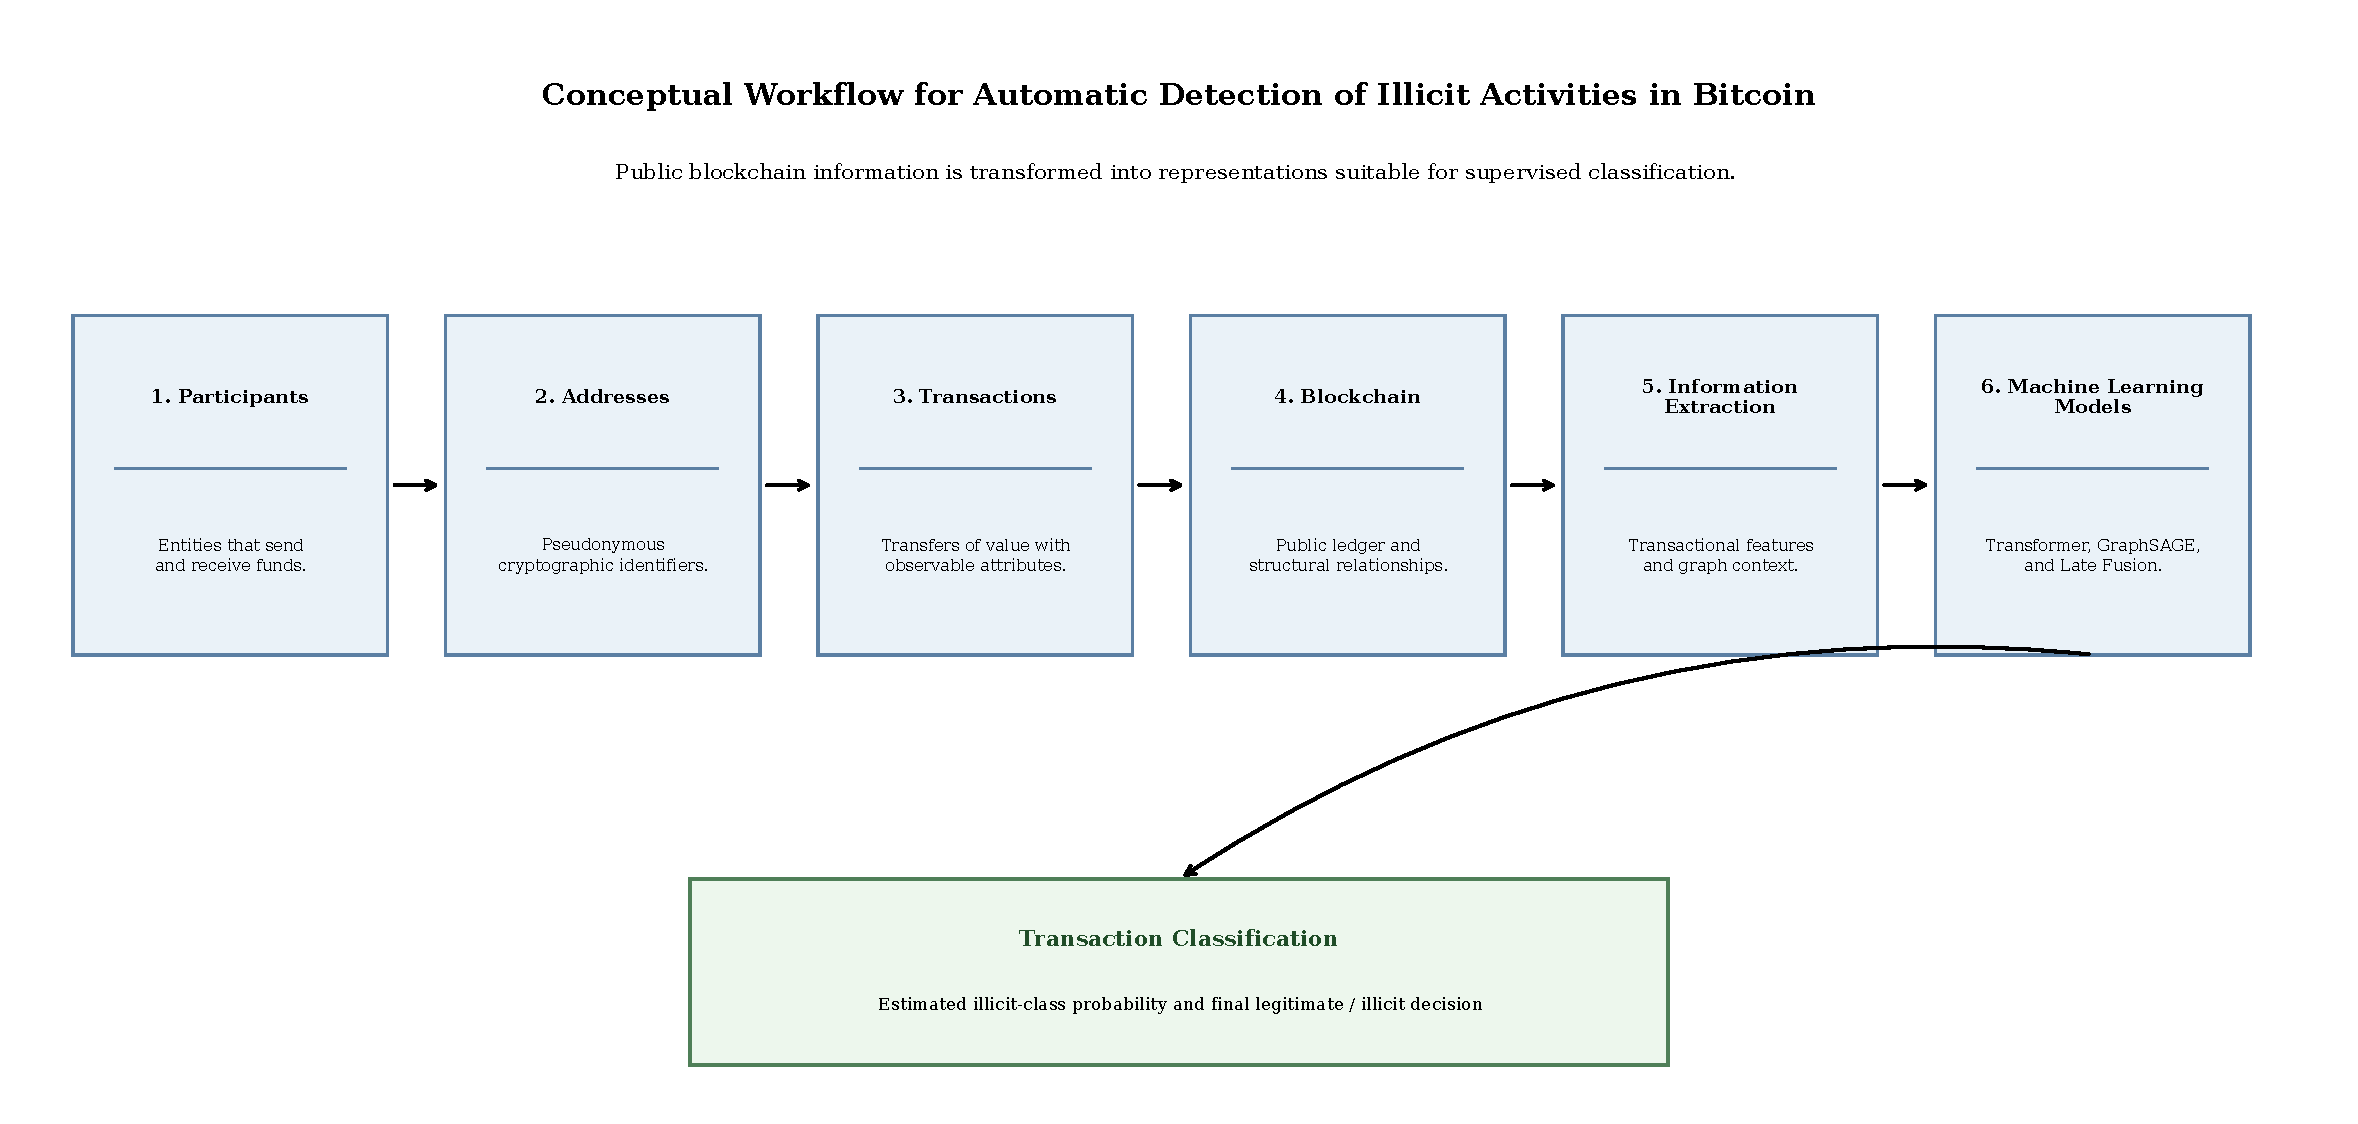
\includegraphics[width=0.98\textwidth]{figures/fig01_problem_overview.pdf}
\caption{Conceptual representation of the Bitcoin anti-money-laundering classification problem.}
\label{fig:problem-overview}
\end{figure*}

% Problem-to-method correspondence
\begin{table*}[t]
\centering
\small
\caption{Correspondence between the main challenges of the problem and the methodological components used to address them.}
\label{tab:problem-method-mapping}
\begin{tabularx}{\textwidth}{p{0.20\textwidth}XX}
\toprule
\textbf{Challenge} & \textbf{Consequence} & \textbf{Methodological response} \\
\midrule
Class imbalance & Overall accuracy can hide poor performance on the illicit class. & Imbalance-aware metrics and optimization of the decision threshold. \\
Complex dependencies among attributes & Discriminative patterns may depend on relationships nonlinear interactions among multiple features. & Transformer to model global interactions among transaction features. \\
Structural relationships between transactions & Observations are not independent and their neighborhood may contain relevant information. & GraphSAGE to learn representations from topological context. \\
Complementary information across models & A single representation may omit signals present in other views of the data. & Late Fusion to combine probabilities produced by complementary models. \\
Experimental variability & A single run may produce conclusions that depend on random initialization. & Evaluation with multiple seeds, means, standard deviations and paired statistical tests. \\
Need for verifiable results & Results may be difficult to audit or reproduce independently. & Deterministic asset pipeline, manifest, hashes SHA-256 and reproducibility metadata. \\
\bottomrule
\end{tabularx}
\end{table*}


% Main result tables
\begin{table*}[t]
\centering
\small
\caption{Main performance comparison of the evaluated anti-money-laundering models.}
\label{tab:main-results}
\begin{tabular}{lrrrrr}
\toprule
Model & F1 & MCC & ROC-AUC & PR-AUC & Bal. Acc. \\
\midrule
MLP & 0.5107 $\pm$ 0.0245 & 0.5069 $\pm$ 0.0293 & 0.8501 $\pm$ 0.0144 & 0.4497 $\pm$ 0.0185 & 0.7040 $\pm$ 0.0113 \\
Transformer & 0.5452 $\pm$ 0.0216 & 0.5523 $\pm$ 0.0381 & 0.8401 $\pm$ 0.0166 & 0.5154 $\pm$ 0.0253 & 0.7130 $\pm$ 0.0086 \\
GraphSAGE & 0.4452 $\pm$ 0.0091 & 0.4353 $\pm$ 0.0226 & 0.8339 $\pm$ 0.0220 & 0.4441 $\pm$ 0.0131 & 0.6804 $\pm$ 0.0124 \\
Hybrid Transformer & \textbf{0.5723 $\pm$ 0.0084} & 0.5875 $\pm$ 0.0114 & 0.8374 $\pm$ 0.0108 & 0.5276 $\pm$ 0.0082 & \textbf{0.7175 $\pm$ 0.0042} \\
Transformer + GraphSAGE & 0.4808 $\pm$ 0.0184 & 0.4769 $\pm$ 0.0258 & 0.8386 $\pm$ 0.0213 & 0.4483 $\pm$ 0.0271 & 0.6907 $\pm$ 0.0118 \\
Late Fusion (ours) & 0.5686 $\pm$ 0.0081 & \textbf{0.5880 $\pm$ 0.0124} & \textbf{0.8509 $\pm$ 0.0099} & \textbf{0.5376 $\pm$ 0.0069} & 0.7134 $\pm$ 0.0053 \\
\bottomrule
\end{tabular}
\end{table*}


\begin{table*}[t]
\centering
\small
\caption{Ablation study comparing early- and late-fusion strategies. The final column reports the absolute MCC difference relative to the Hybrid Transformer.}
\label{tab:fusion-ablation}
\begin{tabular}{lrrrrrr}
\toprule
Model & F1 & MCC & ROC-AUC & PR-AUC & Bal.\ Acc. & $\Delta$ MCC \\
\midrule
Hybrid Transformer & \textbf{0.5723 $\pm$ 0.0084} & 0.5875 $\pm$ 0.0114 & 0.8374 $\pm$ 0.0108 & 0.5276 $\pm$ 0.0082 & \textbf{0.7175 $\pm$ 0.0042} & +0.0000 \\
Transformer + GraphSAGE & 0.4808 $\pm$ 0.0184 & 0.4769 $\pm$ 0.0258 & 0.8386 $\pm$ 0.0213 & 0.4483 $\pm$ 0.0271 & 0.6907 $\pm$ 0.0118 & -0.1106 \\
Late Fusion (ours) & 0.5686 $\pm$ 0.0081 & \textbf{0.5880 $\pm$ 0.0124} & \textbf{0.8509 $\pm$ 0.0099} & \textbf{0.5376 $\pm$ 0.0069} & 0.7134 $\pm$ 0.0053 & +0.0005 \\
\bottomrule
\end{tabular}
\end{table*}


\begin{table*}[t]
\centering
\small
\caption{Paired statistical comparison between Late Fusion and the Hybrid Transformer.}
\label{tab:paired-statistics}
\begin{tabular}{lrrr}
\toprule
Metric & Mean difference & Wilcoxon statistic & Rank-biserial correlation \\
\midrule
Bal. Acc. & -0.0041 & 2.0000 & -0.7333 \\
Precision & 0.0175 & 4.0000 & 0.4667 \\
Recall & -0.0088 & 2.0000 & -0.7333 \\
F1 & -0.0037 & 4.0000 & -0.4667 \\
Macro-F1 & -0.0018 & 4.0000 & -0.4667 \\
ROC-AUC & 0.0135 & 1.0000 & 0.8667 \\
PR-AUC & 0.0101 & 0.0000 & 1.0000 \\
MCC & 0.0005 & 6.0000 & 0.2000 \\
\bottomrule
\end{tabular}
\end{table*}


% Main model-comparison figures
\begin{figure*}[t]
\centering
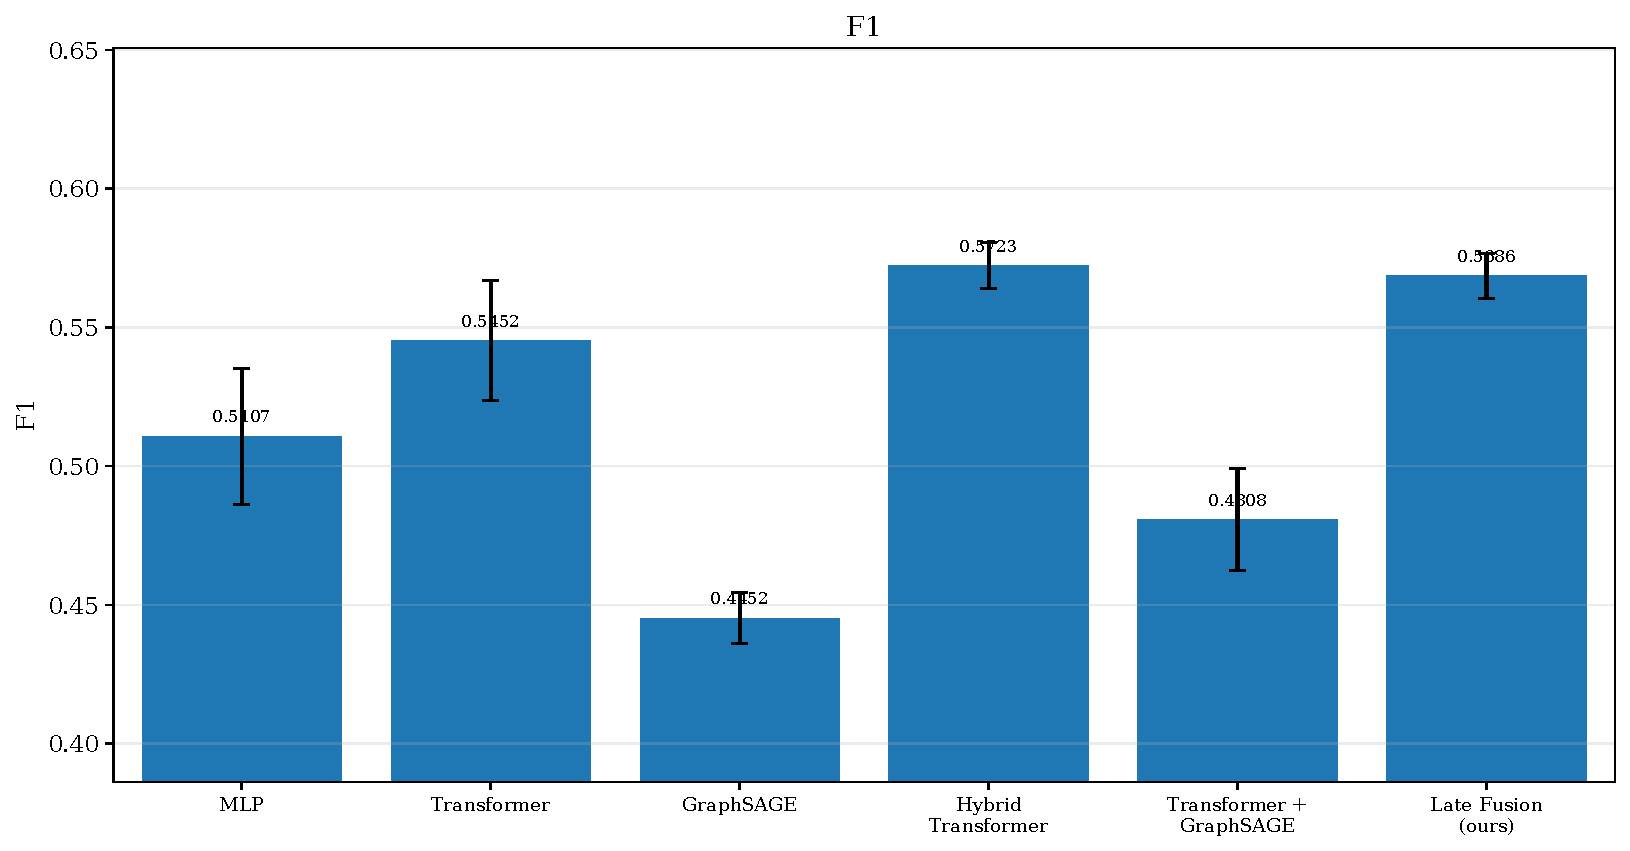
\includegraphics[width=0.48\textwidth]{figures/models_f1.pdf}
\hfill
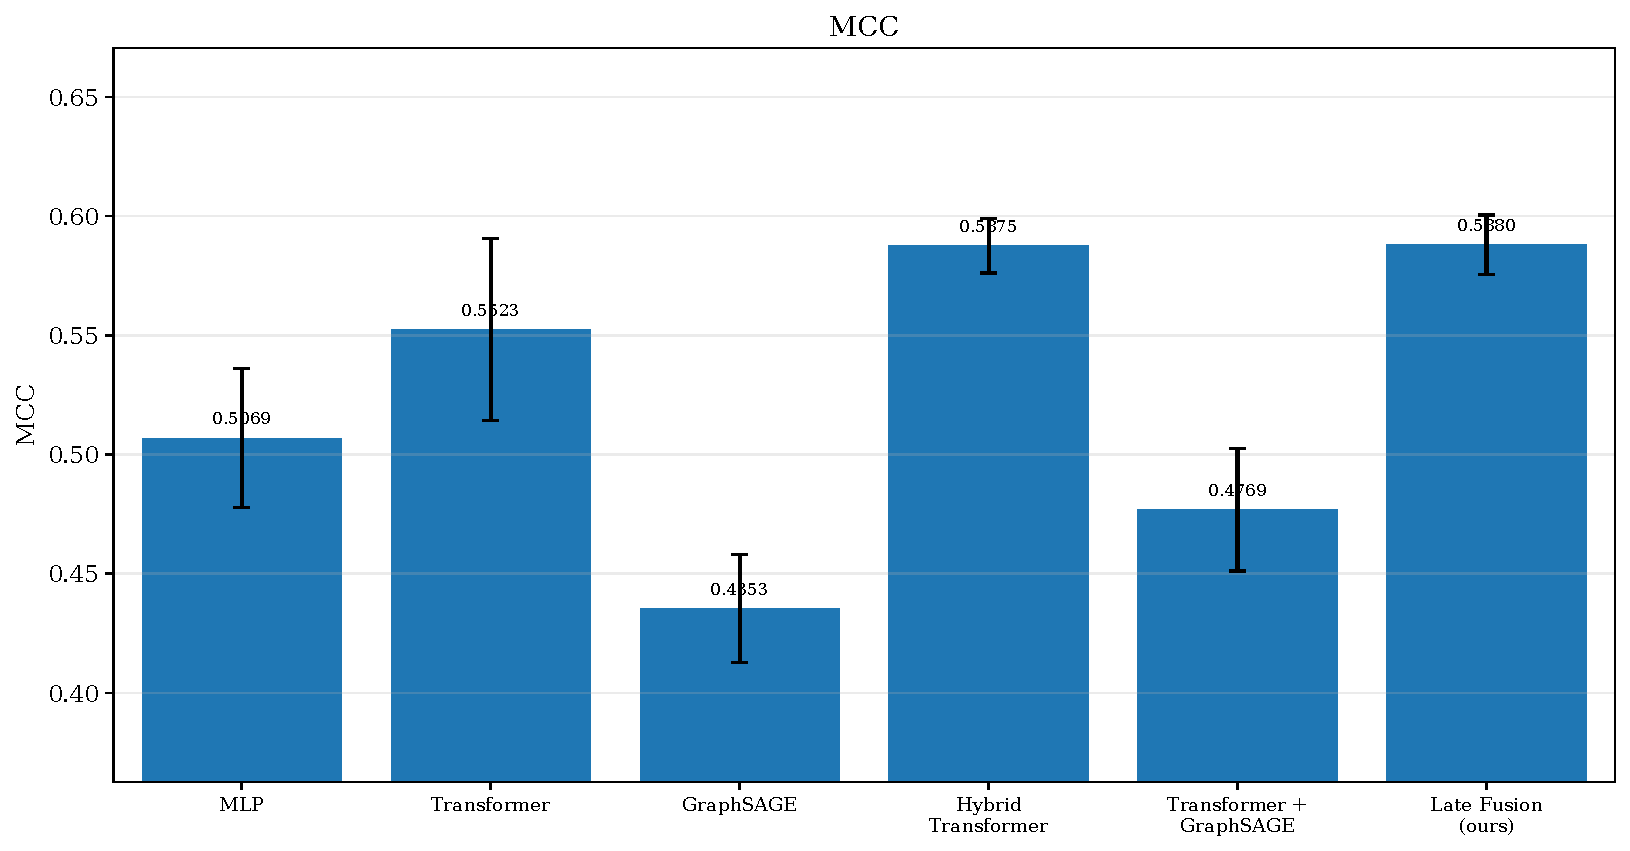
\includegraphics[width=0.48\textwidth]{figures/models_mcc.pdf}
\caption{Comparison of F1 and MCC across the evaluated models.}
\label{fig:model-comparison-f1-mcc}
\end{figure*}

\begin{figure*}[t]
\centering
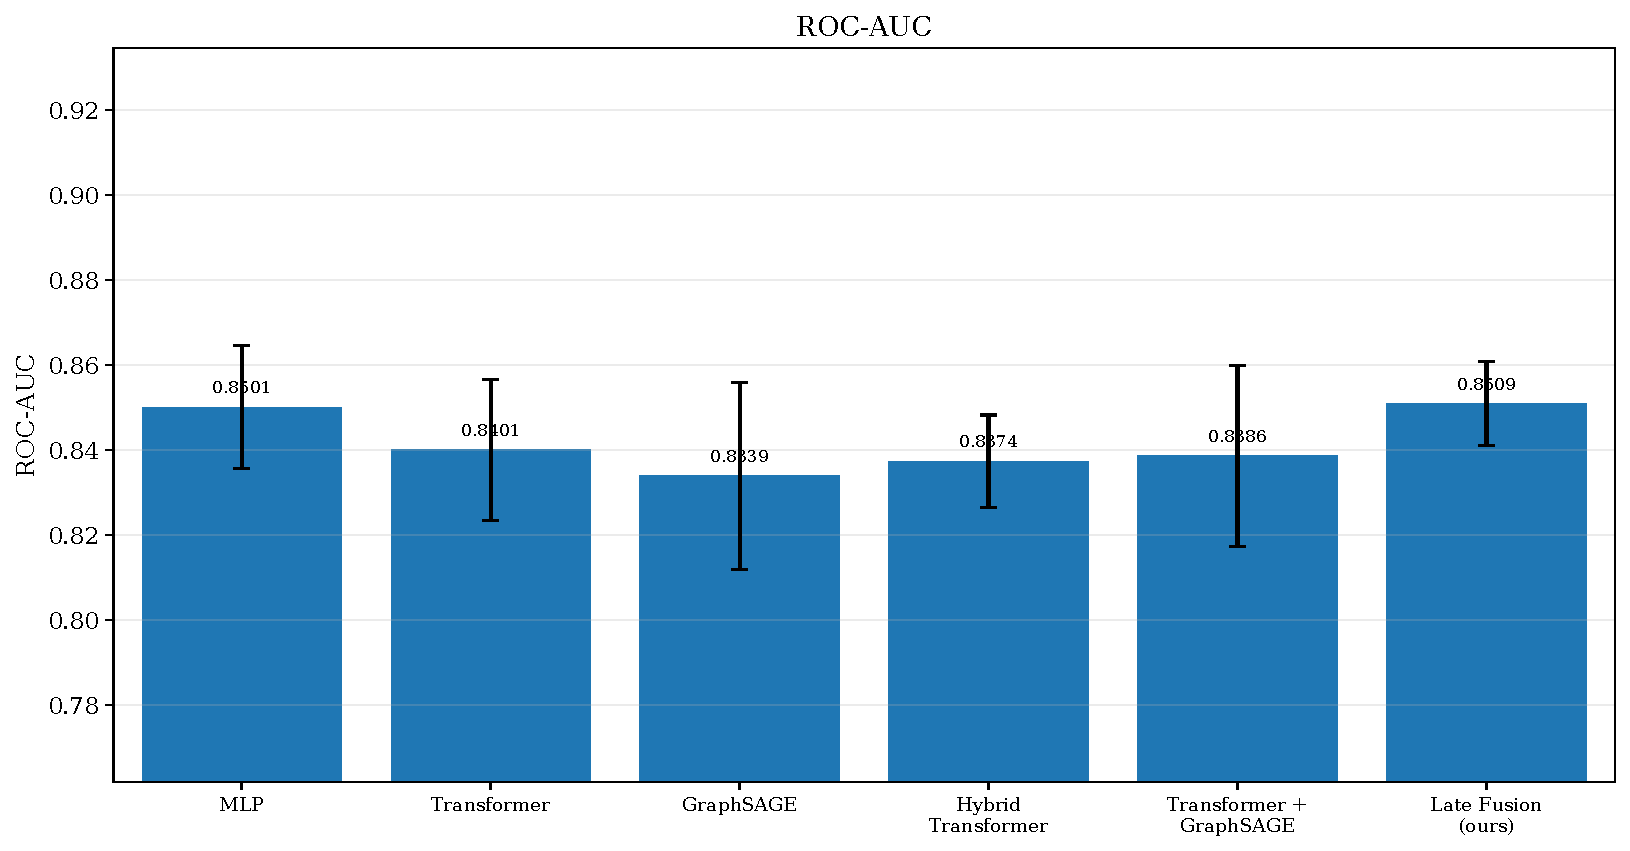
\includegraphics[width=0.48\textwidth]{figures/models_roc_auc.pdf}
\hfill
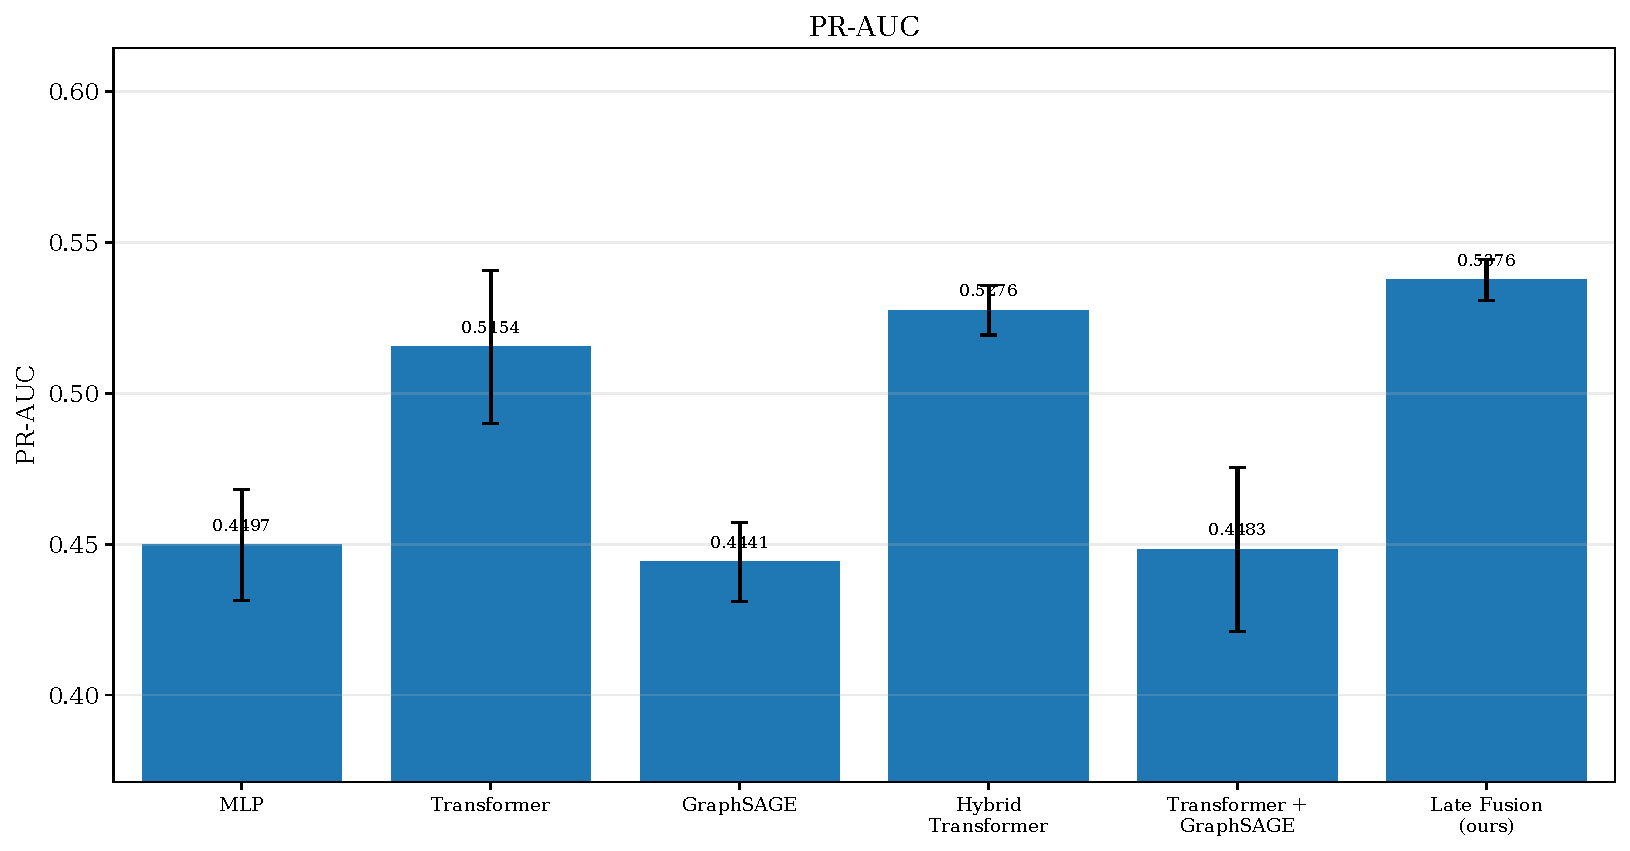
\includegraphics[width=0.48\textwidth]{figures/models_pr_auc.pdf}
\caption{Comparison of ROC-AUC and PR-AUC across the evaluated models.}
\label{fig:model-comparison-auc}
\end{figure*}
